\chapter{Le protocole IPv6}\label{ch:ipv6}

\section{Présentation}
\subsection{Pourquoi l'IPv6 ?}
Le protocole IPv6 succède au protocole IPv4. Celui-ci a été conçu par l'Internet Enginnering Task Force (IETF) pour surmonter les manques de l'IPv4. L'IPv6 apporte notamment :
\begin{itemize}
\item Beaucoup plus d'adresses IP possibles  (avec un maximum de 667 millions de milliards d'appareils connectés sur chaque millimètre carré de la surface de la Terre !). 
    
    \begin{figure}[h]
    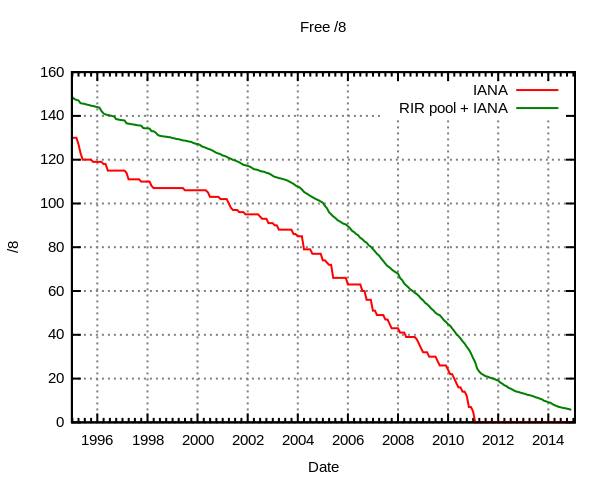
\includegraphics[width=250px]{figures/ipv4-exhaust.png}
    \centering
    \caption{Quantité d'adresse IPv4 disponibles au cours du temps}
    \end{figure}

\item L'implémentation directe de la Quality of Service (QoS \ref{ch:qos});
\item L'implémentation d'un protocole de sécurité (IPSec);
\item Le multicast;
\item La simplification de l'entête des paquets.
\end{itemize}


\subsection{Difficultés rencontrées}
L'IPv6 est incompatible avec l'IPv4 rendant compliqué son déploiement sur Internet. Les hôtes doivent donc proposer une \textit{double pile}, c'est à dire que les appareils disposent à la fois d'une adresse IPv4 et d'une IPv6.
    \begin{figure}[h]
    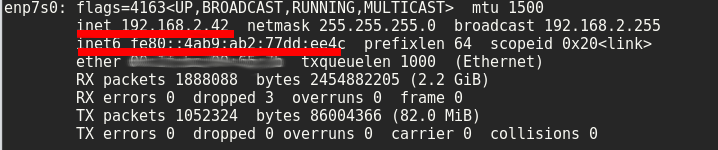
\includegraphics[width=250px]{figures/doubleStack.png}
    \centering
    \caption{Exemple de double pile sur mon ordinateur}
    \end{figure}
    
L'IPv6 étant une technologie encore jeune, les entreprises doivent également éduquer l'ensemble du personnel informatique ralentissant et compliquant la procédure de migration de IPv4 à IPv6 dans les grandes entreprises en plus de la rendre chère.

\section{Types d'adresses IPv6}

\begin{table}[!h]
  \centering
  \begin{tabular}{|l|l|} 
   \hline
    \textbf{Préfixe} & \textbf{Description} \\
    \hline
    ::/8 & Adresses réservées  \\
    \hline
    2000::/3 & Adresses unicast routables sur Internet  \\
    \hline    
    fc00::/7 & Adresses locales uniques  \\
    \hline    
    fe80::/10 & Adresses locales lien  \\
    \hline    
    ff00::/8 & Adresses multicast  \\
    \hline
  \end{tabular}
  \caption{Les différents types d'adresses IPv6.}
\end{table}
\textit{NB: On utilise la notation CIDR pour l'IPv6, de la même facon qu'avec l'IPv4.}

Nous allons désormais expliciter les différents types d'adresses ainsi que leurs utilitées.

\subsection{Les adresses réservées}

Certaines adresses IPv6 sont reservées pour une utilisation particulière : il en existe 13\cite{ReservedAddress}. On pourra noter les plus importantes :
\begin{table}[!h]
  \centering
  \begin{tabular}{|l|p{15cm}|} 
   \hline
    \textbf{Adresse} & \textbf{Description} \\
    \hline
    ::/128 & Adresse non spécifiée. Elle correspond à 0.0.0.0 en IPv4.  \\
    \hline
    ::1/128 & Boucle locale. Elle correspond à 127.0.0.1 en IPv4.  \\
    \hline
    2002::/16 & 6to4.\cite{6to4}. Mécanisme permettant d'envoyer des paquets IPv6 sur un réseau ne supportant que l'IPv4. \\
    \hline
    
  \end{tabular}
  \caption{Quelques adresses IPv6 réservées.}
\end{table}

\subsection{Les adresses unicast}
À la grande différence de l'adressage IPv4, il n'y a plus d'adresse de Broadcast (diffusion) en IPv6.
On pourra retrouver les adresses Unicast, Multicast et Anycast.\\

L' adresse Unicast sert à définir un hôte particulier. Un paquet émis avec cette adresse de destination n'est remis qu'à la machine ayant cette adresse IPv6.\\

IPv6 inclut deux assignations différentes d'adresses unicast :
\begin{itemize}
\item adresse unicast globale;
\item adresse lien local.
\end{itemize}
  
En IPv6, les adresses unicast se présentent ainsi :

\begin{table}[!h]
  \centering
  \begin{tabular}{|l|l|l|l|} 
   \hline
    \textbf{Champ} & Préfixe & Sous-réseau & Interface \\
    \hline
    \textbf{Bits} & \textit{48} & \textit{16} & \textit{64} \\
    \hline
  \end{tabular}
  \caption{Le format d'une adresse unicast. \cite{OracleUnicast}}
\end{table}

Les adresses en lien local sont toujours dans \textit{fc00::/7}.

\subsection{Les adresses multicast}\label{sc:@multicast}

L'adresse de Multicast concerne un ensemble d'hôtes appartenant à un même groupe de diffusion. Un paquet émis avec cette adresse de destination est remis à l'ensemble des machines concernées par cette adresse.\\

En IPv6, les adresses multicast se présentent ainsi :

\begin{table}[!h]
  \centering
  \begin{tabular}{|l|l|l|l|l|} 
   \hline
    \textbf{Champ} & Préfixe & Drapeau & Portée & Groupe \\
    \hline
    \textbf{Bits} & \textit{8} & \textit{4} & \textit{4} & \textit{112} \\
    \hline
  \end{tabular}
  \caption{Le format d'une adresse multicast. \cite{OracleMulticast}}
\end{table}

\subsection{Les adresses anycast}

L'adresse Anycast est ni plus ni moins de l'adressage multicast, à la différence qu'un paquet émis avec cette adresse de destination ne sera remis qu'à un seul membre du groupe. \\
Pour l'instant, une seule adresse anycast est définie et est réservée au routeur mais dans l'avenir, d'autres pourraient être définies. \\
La construction d'une adresse IPv6 anycast d'un sous-réseau (la seule définie actuellement) concatène le préfixe du sous réseau de l'interface et la valeur nulle pour la dernière partie de l'adresse.

\begin{table}[!h]
  \centering
  \begin{tabular}{|c|c|} 
   \hline
	\textit{n bits} & \textit{112 - nbits} \\
    \hline
    {Préfixe de sous-réseau} & {ID du groupe} \\
    \hline
  \end{tabular}
  \caption{Le format d'une adresse anycast.}
\end{table}
